\section{MPLS Signatures Validation}\label{validation}
% %%%%%%%%%%%%%%%%%%%%%%%%%%%%%%%%%%%%
\begin{figure}[!t]
  \begin{center}
    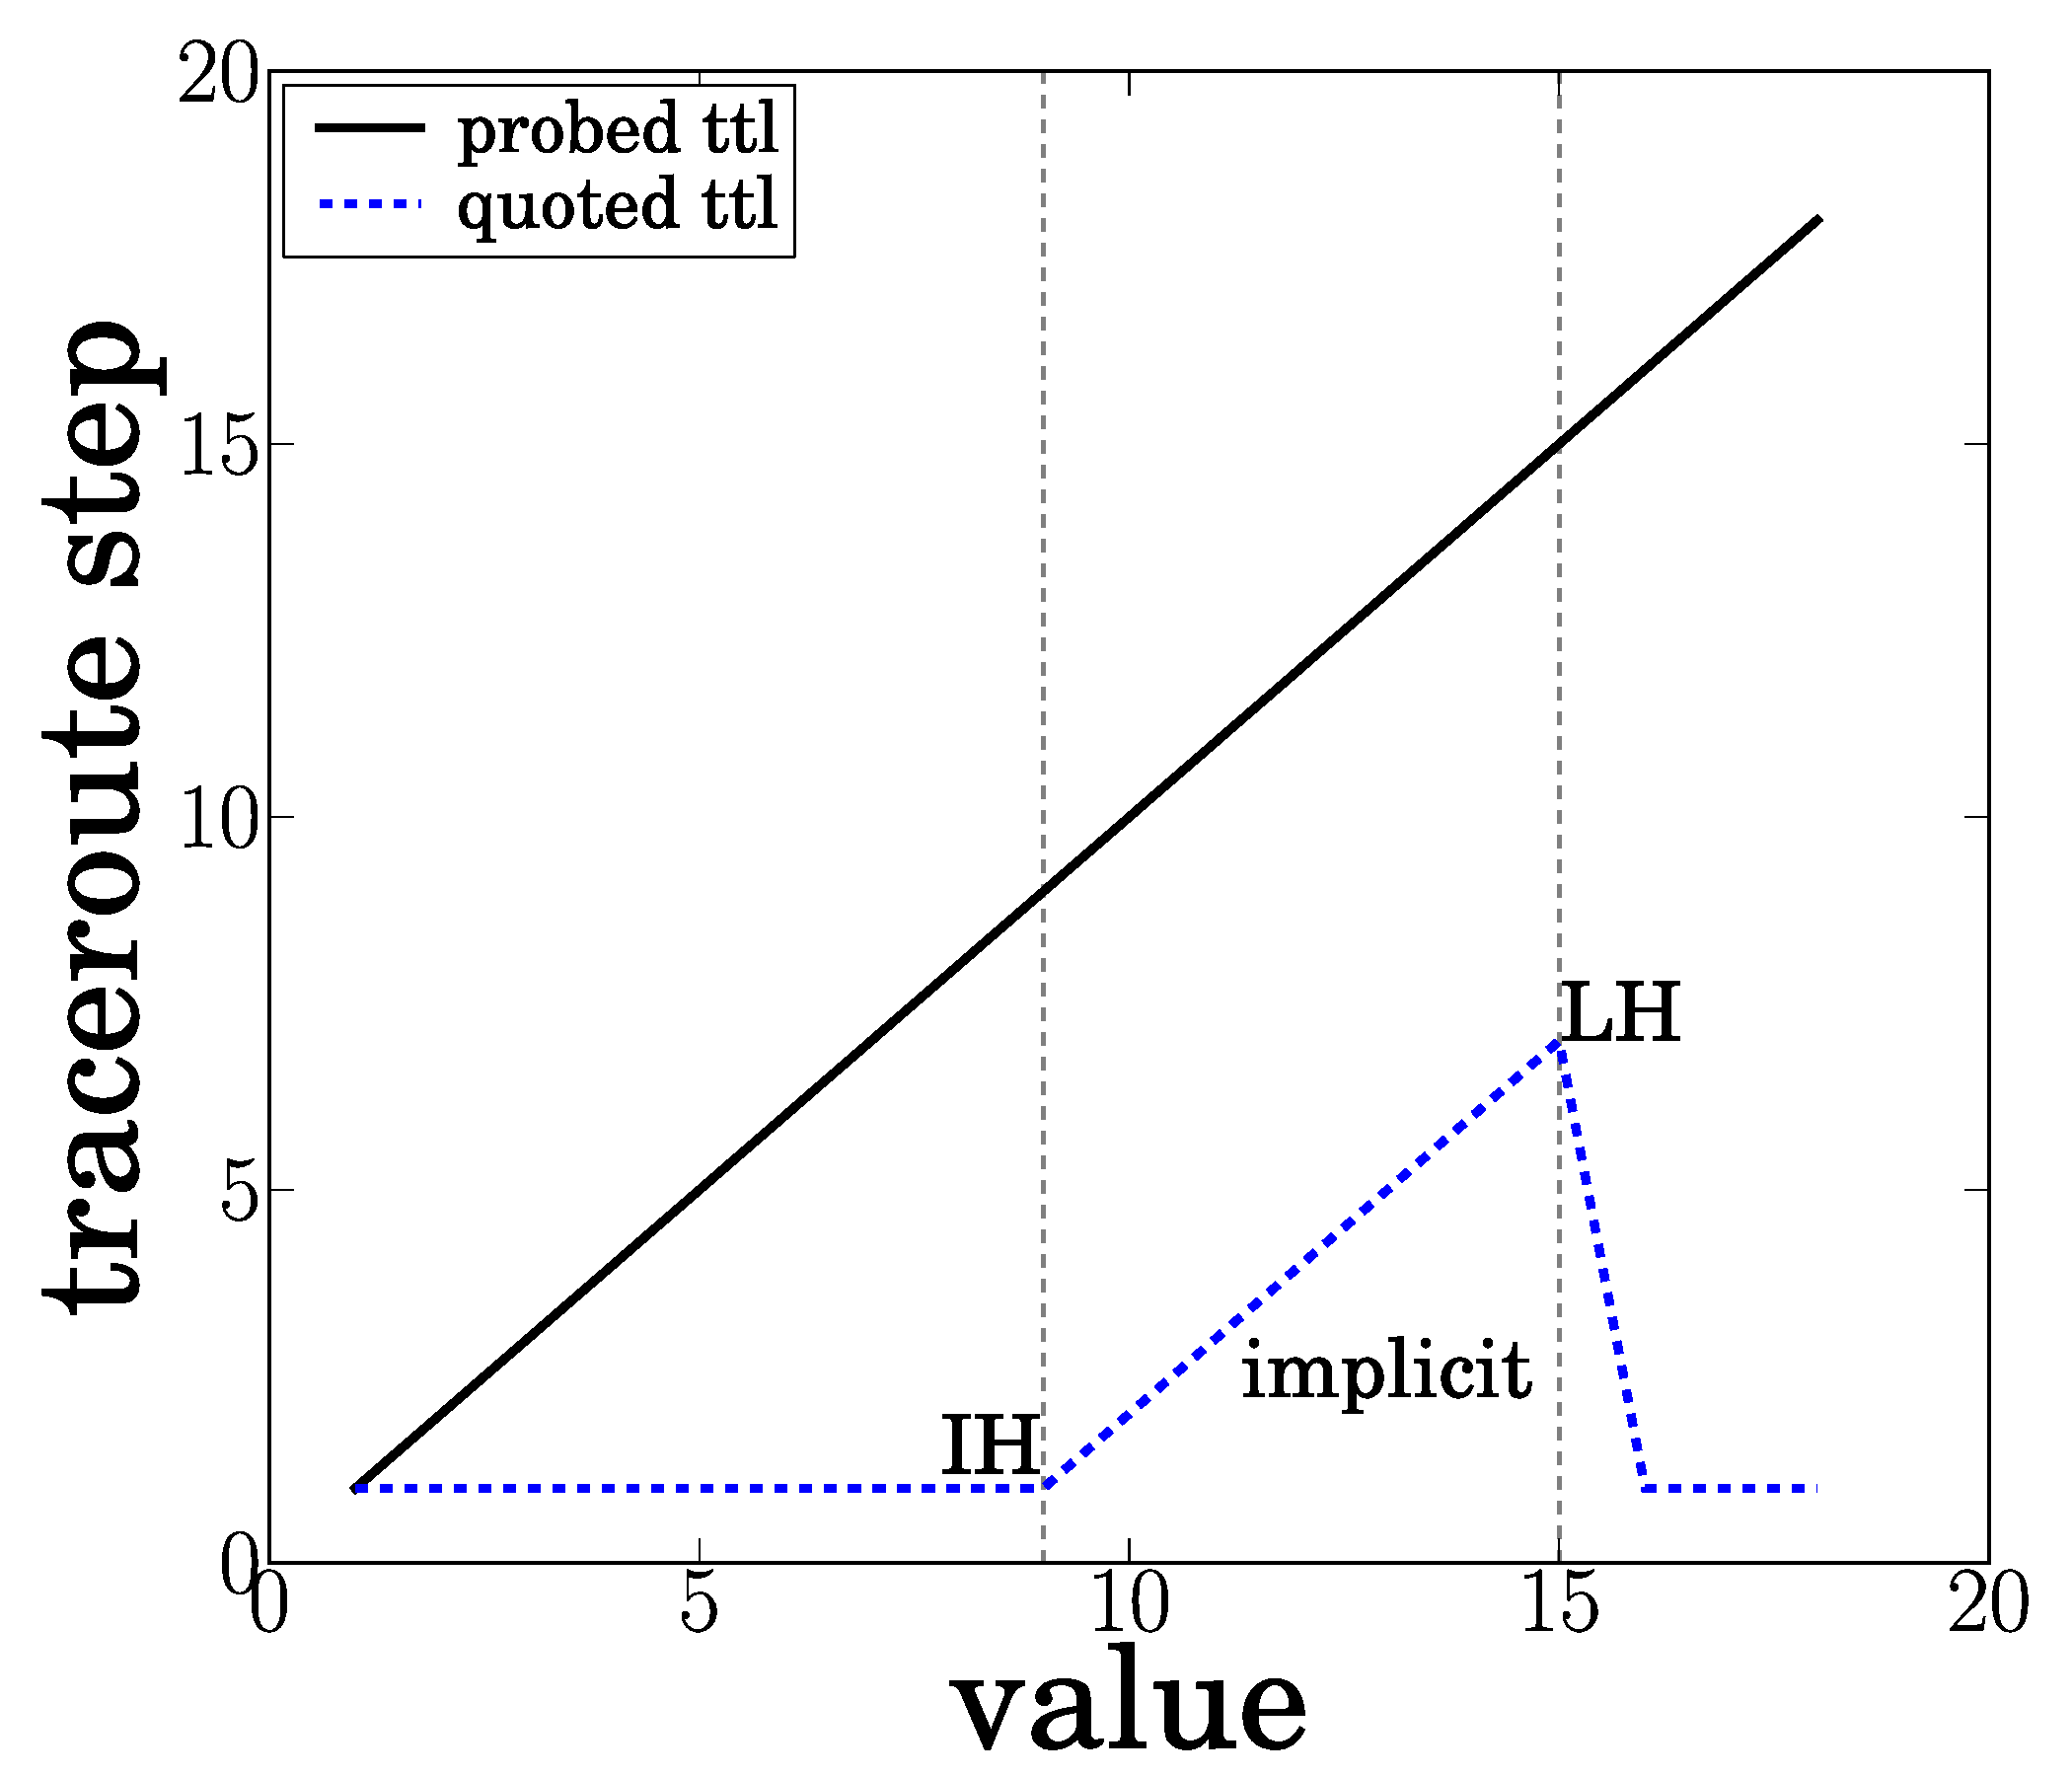
\includegraphics[width=4cm]{QuotedTTL}
  \end{center}
  \caption{Example of qTTL signature for an implicit MPLS tunnel.}
  \label{validation.qTTLFig}
\end{figure}

In this section, we expose our methodology for validating the MPLS
signatures used to reveal implicit MPLS tunnels (see Sec.~\ref{related.revealing}).
Basically, we compare the LSR position within an MPLS tunnel, called the
\dfn{MPLS position}, with the different signatures values. 

Implicit tunnels are based either on qTTL or u-turn signatures. Both of them are
directly related with MPLS position.  Indeed, first, the qTTL value refers to
the IP-TTL of the \echorequest packet when it enters the MPLS tunnel. 
Therefore, a qTTL of $n$ in the resulting ICMP \ttlexceeded means that the sent
probe expired $n$ hops later than the Ingress LER of the LSP, i.e., an LSR reply
with qTTL$=n$ means that the LSR appears in the \dfn{$n$-position} in the LSP. 
This is illustrated in Fig.~\ref{validation.qTTLFig}.  From the Ingress LER, the
qTTL starts to grow linearly with the LSP length.  We therefore expect observing
a qTTL=$1$ on the first LSR in the LSP, a qTTL$=2$ on the second LSR in the LSP,
etc.  Second, a u-turn value is related to the tunnel length, $L$, and the
$n$-position of the LSR within the tunnel (see Sec.~\ref{related.revealing}).

\subsection{qTTL Signature}\label{validation.qttl}
%%%%%%%%%%%%%%%%%%%%%%%%%%%
\begin{figure}[!t]
  \begin{center}
    \subfigure[Tunnel length distribution]{\label{hist_length}
      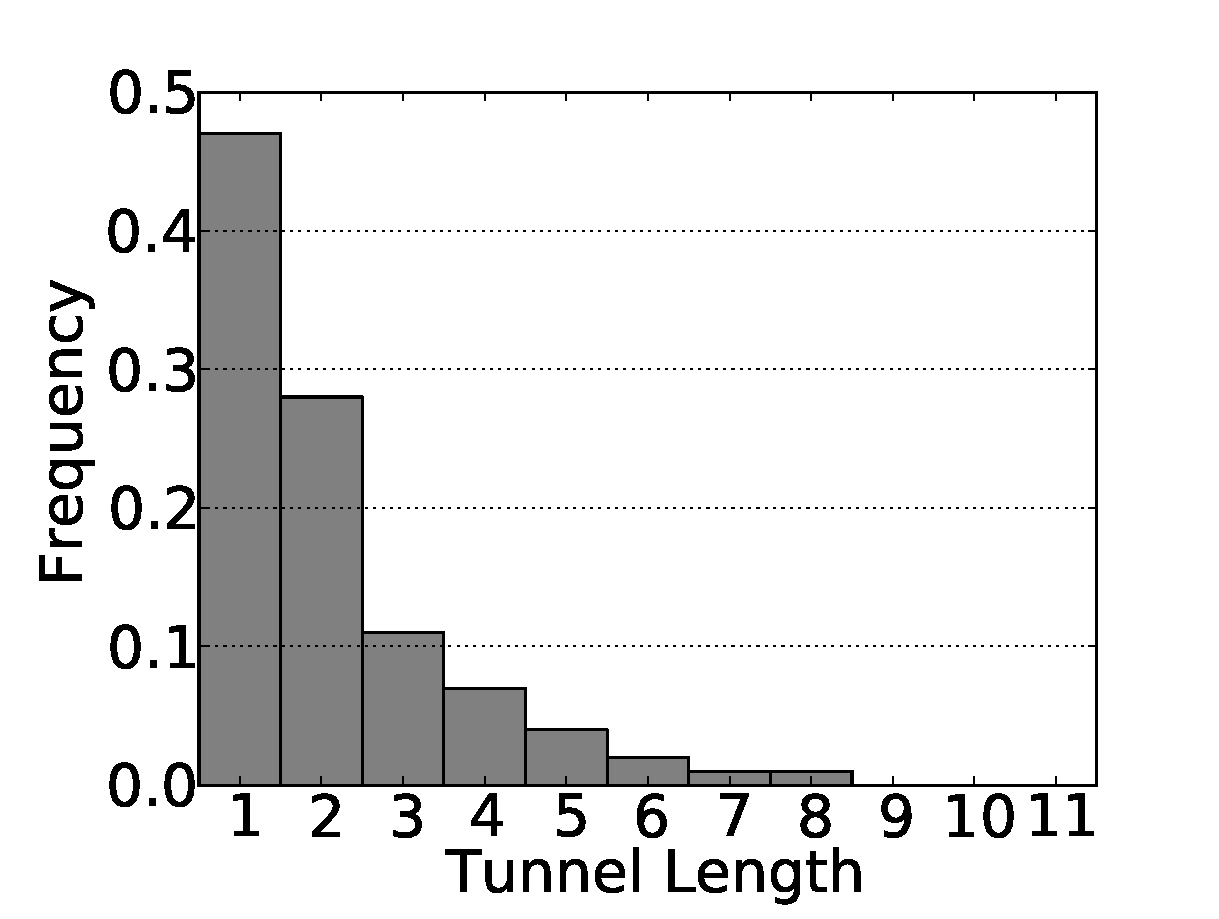
\includegraphics[width=4.3cm]{hist_length}}
\hspace{-0.3cm}      
    \subfigure[qTTL and $n$-position comparison]{\label{n_vs_qttl}
      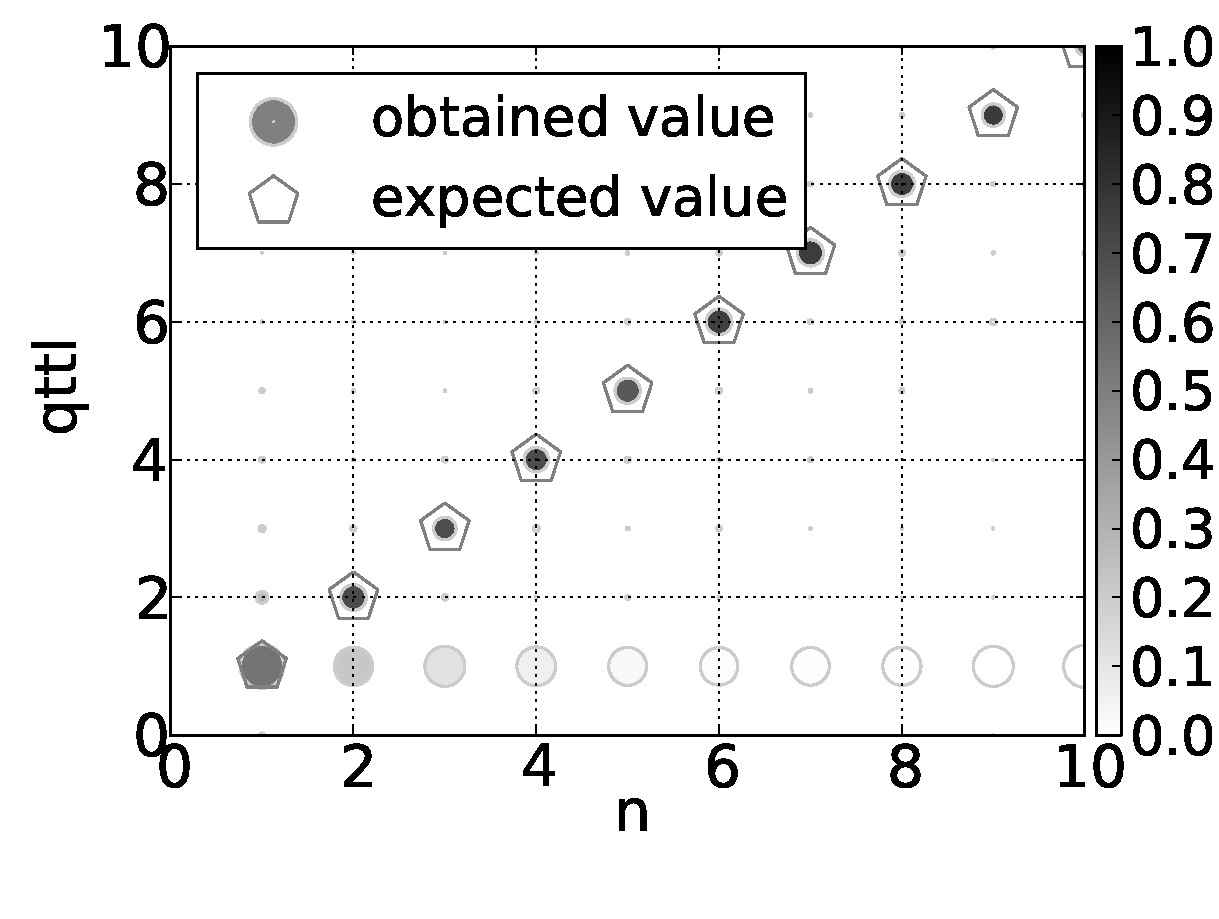
\includegraphics[width=4.3cm]{n_vs_qttl}}  
  \end{center}
  \caption{Comparison between obtained and expected values for qTTL and u-turn.}
  \label{validation.qttl.fig}
\end{figure}

Our signature validation relies on the hypothesis that the MPLS position matches
with the $n$-position, i.e., the position of the LSR within the LSP (MPLS
position) corresponds to the qTTL value generated by that LSR ($n$-position). 
Said differently qTTL = $n$.

In order to validate this assumption, we use the dataset described in
Sec.~\ref{dataset} and compare the qTTL with $n$ for implicit tunnels
\ed{correct?}. The results are shown in Fig.~\ref{validation.qttl.fig}.  In
particular, Fig.~\ref{hist_length} provides the MPLS tunnel length distribution
computed as the number of LSRs in the tunnel.  We observe, confirming so
previous studies~\cite{SOM11,Vanaubel15,Donnet12}, that most of tunnels are
rather short (length $< 3$ in more than 80\% of the cases). 
Fig.~\ref{hist_length} also provides, by extension, possible values for qTTL
(X-axis).  This suggests thus that qTTL values should oscillates between 1 and
8, with a strong predominance for short values (i.e., between 1 and 3).

Fig.~\ref{n_vs_qttl} represents a scatter plot showing the relations between the
qTTL (Y-axis) and the $n$-position (X-axis).  The circle size in the scatter
plot is related with the occurrence frequency of Y-axis values regarding each
$n$-position.  The transparency of the circle is related with occurence
frequency of the $n$-position regarding each Y-axis value.  For instance, on
Fig.~\ref{n_vs_qttl} for values where $n>1$, the biggest circles are mainly
located on qTTL$=1$ and qTTL=$n$.  So, this suggests that, for a given
$n$-position, the qTTL value usually takes either the value $1$ or $n$.

However, we notice, on Fig.~\ref{n_vs_qttl} that the qTTL signature highly
matches with $n$.   The bias $\textit{qTTL}=n \pm \epsilon$ could occur due to
two causes: one is the limitation in our method to reveal the first LSR in the
LSP when RFC4950 is not implemented (by definition of implicit tunnel); and the
second cause could occur due to load balancers (using Paris traceroute should
avoid load balancing issues, except for ``per packet'' load balancers).
In the later case, the \traceroute probes may follow paths with different
lengths before reaching the MPLS tunnel, yielding that the same qTTL value is
revealed several times in different $n$-positions. Fig.~\ref{n_vs_qttl} also
shows that qTTL frequently takes the value of $1$, which is consistant with
tunnel length distribution (see Fig.~\ref{hist_length}).  

We also find that around $2\%$ of LSRs do not react to qTTL signature, even
if \tpropagate option is activated, i.e., some LSRs interfaces located at
$i_{n \pm 1}$ tunnel positions react properly to qTTL signatures but the LSR
interface located at $i_n$ position does not.

% This usually  means that \tpropagate is not implemented \ed{we are not anymore
% in the case of an implicit tunnel, no?}.

Nevertheless, the $n$-position is highly reliable. Indeed, we find that in
$58\%$ of the cases the $n$-position matches with the qTTL value while in
$36,3\%$ of cases the qTTL signature is not present and takes the value of $1$,
and just $6,7\%$ of the cases presented have some bias around the expected value
$n$. Those results support our hypothesis: the  MPLS tunnel position highly
matches with the $n$-position. Thereby,  we use $n$-position as a reference
value to validate the u-turn signatures.

\subsection{u-turn Signature}\label{validation.uturn}
%%%%%%%%%%%%%%%%%%%%%%%%%%%%%%
\begin{figure}[!t]
  \begin{center}    
    \subfigure[u-turn on LSRs revealed through RFC4950 and qTTL]{\label{fig_uturn_a}
      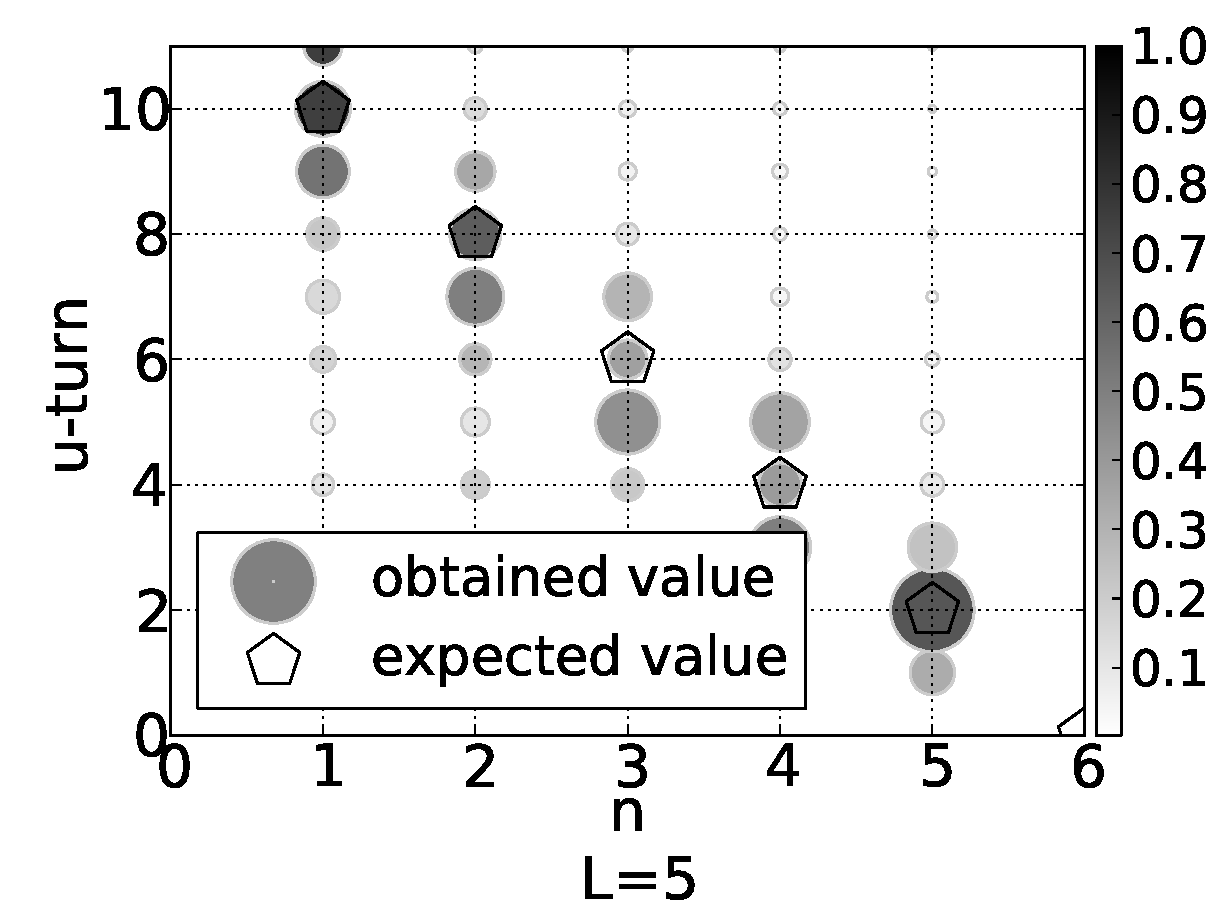
\includegraphics[width=4.3cm]{n_vs_uturn_L5_exp}}
\hspace{-0.3cm}      
    \subfigure[u-turn on LSRs where no other signature was found]{\label{fig_uturn_b}
      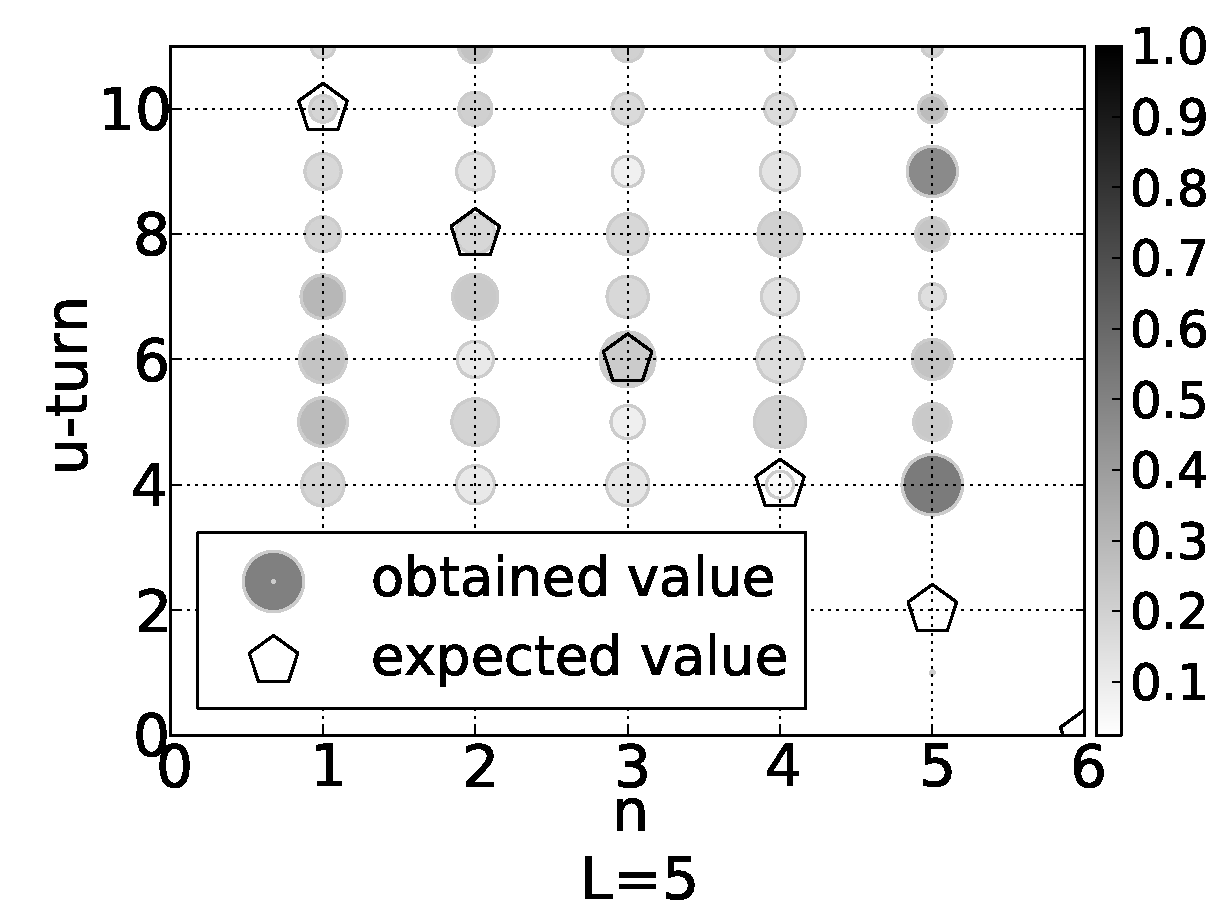
\includegraphics[width=4.3cm]{n_vs_uturn_L5}}
  \end{center}
  \caption{Comparison between obtained and expected values for u-turn
  signature.}
  \label{validation.uturn.fig}
\end{figure}

As explained in Sec.~\ref{related.revealing},  the expected u-turn value is in
the form $[2L, 2L-2, 2L-4,..., 2]$ where $L$ is the tunnel length and the array
position corresponds to the LSR position within the LSP, i.e., $n$.  The
relationship between $L$, $n$, and the expected value can thus be written as
follows:
\begin{equation}
u-turn = 2 \times (L - (n-1)) .
\label{eqn.uturn}
\end{equation}

\ed{This relationship might not look like obvious at first glance.  If we have
room, we should add a figure to illlustrate (as done for qTTL above).}

Because u-turn is commonly present in almost all LSRs, first, we compare $n$
with u-turn on LSRs revealed either explicitly or qTTL-based using the dataset
presented in Sec.~\ref{dataset}.  We also study  $n$ value on LSRs where u-turn
was the only detected signature. We use the filter $\textit{u-turn}>3$ (i.e.,
avoiding so short tunnels where bias are more likely to appear) to avoid false
positives.

The results for a given tunnel length $L=5$ are shown on
Fig.~\ref{validation.uturn.fig}, a scatter plot that must be read the same way
as Fig.~\ref{n_vs_qttl}.  In a few words, Fig.~\ref{validation.uturn.fig}
suggests that u-turn is usually overestimated.  \ed{I stopped here (next
should be rephrased) as I was running out of time.}


 and Fig.~\ref{fig_uturn_b}. Similar results
where also obtained for other tunnel length $L$ values. Basically, we noticed
that the percentage of cases \ed{cases of what?} are close to expected ones when
the LSRs explicitly revealed \ed{revealed what?} and qTTL is present
(Fig.~\ref{fig_uturn_a}). However, on the set of LSRs revealed just by u-turn
signatures (Fig.~\ref{fig_uturn_b}) the cases \ed{again, the cases of what?}
commonly does not match. If we accept a bias of $ \pm 1$ around the expected
value \ed{of what?}, we noticed that on LSRs explicitly revealed and qTTL
signature based, the $60\%$ of obtained u-turn signed cases match with the
expected values \ed{again, of what?}. However, on LSRs revealed just trough
u-turn signature (therefore where it is really useful), the obtained u-turn
cases just match in $25\%$ with the expected value $2(L-(n-1))$.
Therefore, LSRs revealed \ed{only?} through u-turn is highly inaccurate; mainly
because MPLS tunnels are not the only responsible on the variation in it length,
but also the load balancing is common for paths between the same pairs
source-destination \cite{BRICE07}. This issue is called \dfn{per-flow} load
balancing. Basically, packets that belongs to the same \dfn{flow} are treated
similarly \cite{BRICE06}. A flow is identified by the first 32 bits of the IP
\textit{payload}, e.g., TCP header. In the case of ICMP messages, this fields
refers to \texttt{Type}, \texttt{Code}, and \texttt{Checksum}.
By definition, u-turn signature is based on two kinds of ICMP messages:
ICMP \echoreply \texttt{Code 11} and ICMP \ttlexceeded \texttt{Code 0}.
Due to different codes for each ICMP message, there is no way to assure that
they belong to the same flow identifier and thereby to be sure that u-turn value
is caused just by MPLS tunnels.  \ed{The full explanation of ``per flow'' is not
required (we can assume people are familiar with this).  But we have to clearly
state that this is during the ``return'' path (i.e., from the LSR generating the
\ttlexceeded towards the VP) that those per-flow LB can mainly occur.
Otherwise, I miss something here.}
